\documentclass[a4paper,12pt]{article}

\usepackage{school}

\begin{document}
    \head{21 декабря}{Трёхмерные движения и симметрии}
    
    \section{Разбор}
    
    \defn \emph{Трёхмерным движением} называется преобразование трёхмерного пространства $F\colon \R^3 \to \R^3$, сохраняющее расстояния
    \begin{equation*}
        \forall x,y \in \R^3 \Big(\dist(x, y) = \dist(F(x), F(y))\Big).
    \end{equation*}
    Для краткости, в этом листке мы будем называть их просто движениями.
    \example Отражение относительно плоскости $H \subset \R^3$.
    \example Параллельный перенос на вектор $\bar{v}$.
    \example Поворот вокруг оси $l \subset \R^3$ на угол $\alpha \in [0^\circ,360^\circ)$.
    
    \defn \emph{Симметрией} трёхмерной фигуры $\Phi \subset \R^3$ называется движение $F\colon \R^3 \to \R^3$, оставляющее фигуру на месте
    \begin{equation*}
        \forall x \in \Phi \ (F(x) \in \Phi).
    \end{equation*}
    \problem Множество всех симметрий фигуры является группой относительно операции композиции.
    
    \defn \emph{Флагом} для многогранника $\Phi$ называется тройка $(V, E, F)$, где $V$ --- вершина $\Phi$, $E$ --- ребро $\Phi$, смежное с $V$, а $F$ --- грань $\Phi$, смежная с $E$.
    \problem Пусть $\Phi$ --- любой многогранник, а $(V, E, F)$ --- любой флаг в нём. Покажите, что единственная симметрия $\Phi$, оставляющая этот флаг на месте --- тождественная.
    
    \begin{wrapfigure}{r}{0.4\linewidth}
        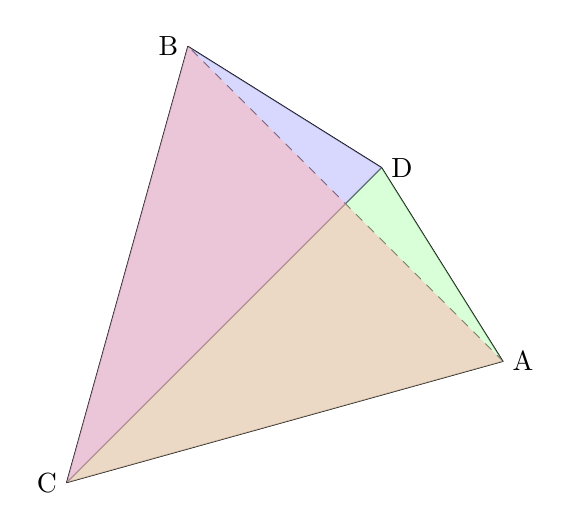
\begin{tikzpicture}[line join=round, line cap=round, scale=4]
            \coordinate [label=right:A] (A) at (1,0,0);
            \coordinate [label=left:B] (B) at (0,1,0);
            \coordinate [label=left:C] (C) at (0,0,1);
            \coordinate [label=right:D] (D) at (1,1,1);
            
            \draw[dashed] (A) -- (B);
            \draw (A) -- (C) -- (D) -- (B) -- (C) (A) -- (D);
            
            \fill[green!30, opacity=.5] (A)--(D)--(C)--cycle;
            \fill[blue!30, opacity=.5] (B)--(D)--(C)--cycle;
            \fill[red!30, opacity=.5] (B)--(A)--(C)--cycle;
        \end{tikzpicture}
    \end{wrapfigure}
    \problem Пусть $G$ --- группа симметрий тетраэдра. \\
    \sub Сколько элементов в $G$? \\
    \sub Найдите какое-нибудь множество образующих $G$. \\
    \sub Какие перестановки вершин они реализуют? \\
    \sub Сколько из них отражений, поворотов, переносов? \\
    \sub Какие перестановки рёбер они реализуют? \\
    \sub Какие перестановки граней они реализуют?
    \begin{solution}
        \sub Заметим, что отражение относительно серединно-перпендикулярной плоскости к ребру тетраэдра (например, $AB$) является симметрией. Будем обозначать такую симметрию $s_{**}$ (например, $s_{AB}$). Ясно, что $s_{AB}$ оставляет на месте ребро $CD$, а вершины $A$ и $B$ меняет местами. Пользуясь такими симметриями можно перевести любой флаг в тетраэдре в любой другой. Следовательно, элементов в $G$ столько же, сколько и флагов, то есть $4 \cdot 3 \cdot 2 = 24$. \\
        \sub Из предыдущего пункта ясно, что $\{s_{AB}, s_{AC}, s_{AD}, s_{BC}, s_{BD}, s_{CD}\}$ --- множество образующих. \\
        \sub Образующие из предыдущего пункта реализуют все транспозиции вершин. Так как любая перестановка может быть записана произведением транспозиций, любая перестановка реализуется какой-нибудь симметрией. \\
        \sub Транспозиции (6 штук) реализуются отражениями. Перестановки типа $\cycle{A,B,C}$ (8 штук) реализуются поворотами на $\pm 120^\circ$ относительно высоты, проведённой из точки $D$ к плоскости $ABC$. Перестановки типа $\cycle{A,B}\cycle{C,D}$ (3 штуки) реализуются поворотами на $180^\circ$ относительно прямой, проходящей через середины $AB$ и $CD$. Остались перестановки типа $\cycle{A,B,C,D}$ (6 штук). Покажем, что они не являются ни отражениями, ни поворотами, ни переносами. Перенос вообще не может быть симметрией, так как не оставляет на месте центр тетраэдра. Отражение всегда имеет порядок 2, так что не может реализовывать перестановку порядка 4. Поворот не перемешивает точки из разных плоскостей, перпендикулярных своей оси. Следовательно, если бы эта перестановка реализовывалась поворотом, то все 4 вершины тетраэдра должны были бы лежать в одной плоскости, что неверно. Итого: 6 отражений, 11 нетривиальных поворотов, 0 нетривиальных переносов. \\
        \sub Рёбра тетраэдра можно разбить на три пары противоположных: $AB$ и $CD$, $AC$ и $BD$, $AD$ и $BC$. Ясно, что противоположные рёбра останутся таковыми. Заметим, что симметрия $s_{AB}$ реализует перестановку рёбер $\cycle{AD,BD}\cycle{AC,BC}$. Так как такие симметрии порождают нашу группу, любая перестановка рёбер, реализуемая симметрией, является чётной. Вместе с предыдущим условием это выделяет как раз 24 различных перестановки. \\
        \sub Симметрия $s_{AB}$ реализует транспозицию граней. Следовательно, аналогично вершинам, можно получить любую перестановку граней.
    \end{solution}  
    
    \section{Задачи для самостоятельного решения}
    
    \problem Пусть $G$ --- группа симметрий куба. \\
    \sub Сколько элементов в $G$? \\
    \sub Найдите какое-нибудь множество образующих $G$. \\
    \sub Какие перестановки вершин они реализуют? \\
    \sub Сколько из них отражений, поворотов, переносов? \\
    \sub Какие перестановки рёбер они реализуют? \\
    \sub Какие перестановки граней они реализуют?
    
    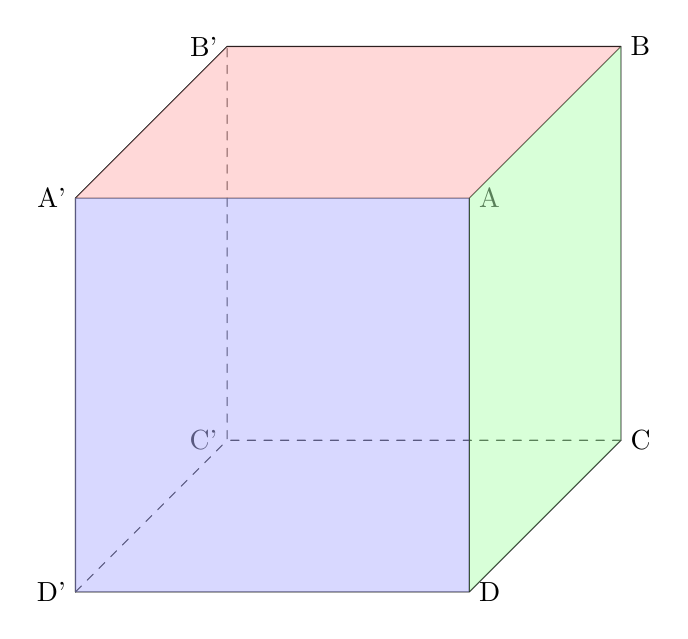
\begin{tikzpicture}[line join=round, line cap=round, scale=2.5]
        \coordinate [label=right:A] (A) at (1,1,1);
        \coordinate [label=right:B] (B) at (1,1,-1);
        \coordinate [label=right:C] (C) at (1,-1,-1);
        \coordinate [label=right:D] (D) at (1,-1,1);
        \coordinate [label=left:A'] (A') at (-1,1,1);
        \coordinate [label=left:B'] (B') at (-1,1,-1);
        \coordinate [label=left:C'] (C') at (-1,-1,-1);
        \coordinate [label=left:D'] (D') at (-1,-1,1);
        
        \draw[dashed] (D')--(C')--(B') (C)--(C');
        \draw (A)--(B)--(C)--(D)--(A)--(A')--(B')--(B) (A')--(D')--(D);
        
        \fill[green!30, opacity=.5] (A)--(B)--(C)--(D)--cycle;
        \fill[blue!30, opacity=.5] (A)--(A')--(D')--(D)--cycle;
        \fill[red!30, opacity=.5] (B)--(B')--(A')--(A)--cycle;
    \end{tikzpicture}
    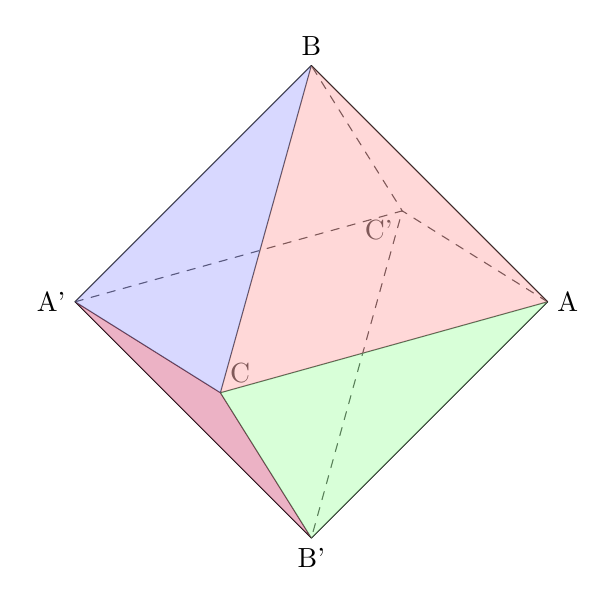
\begin{tikzpicture}[line join=round, line cap=round, scale=3]
        \coordinate [label=right:A] (A) at (1,0,0);
        \coordinate [label=above:B] (B) at (0,1,0);
        \coordinate [label=above right:C] (C) at (0,0,1);
        \coordinate [label=left:A'] (A') at (-1,0,0);
        \coordinate [label=below:B'] (B') at (0,-1,0);
        \coordinate [label=below left:C'] (C') at (0,0,-1);
        
        \draw[dashed] (A')--(C')--(B') (A)--(C')--(B);
        \draw (A)--(B)--(C)--(B')--(A)--(C)--(A')--(B) (A')--(B');
        
        \fill[red!30, opacity=.5] (A)--(B)--(C)--cycle;
        \fill[green!30, opacity=.5] (A)--(B')--(C)--cycle;
        \fill[blue!30, opacity=.5] (A')--(B)--(C)--cycle;
        \fill[purple!60, opacity=.5] (A')--(B')--(C)--cycle;
    \end{tikzpicture}
    
    \problem Пусть $G$ --- группа симметрий октаэдра. \\
    \sub Сколько элементов в $G$? \\
    \sub Найдите какое-нибудь множество образующих $G$. \\
    \sub Какие перестановки вершин они реализуют? \\
    \sub Сколько из них отражений, поворотов, переносов? \\
    \sub Какие перестановки рёбер они реализуют? \\
    \sub Какие перестановки граней они реализуют?
    
    \problem Пусть $G$ --- группа симметрий додекаэдра. \\
    \sub Сколько элементов в $G$? \\
    \sub Найдите какое-нибудь множество образующих $G$. \\
    \sub Какие перестановки вершин они реализуют? \\
    \sub Сколько из них отражений, поворотов, переносов? \\
    \sub Какие перестановки рёбер они реализуют? \\
    \sub Какие перестановки граней они реализуют?
    
    \problem Пусть $G$ --- группа симметрий икосаэдра. \\
    \sub Сколько элементов в $G$? \\
    \sub Найдите какое-нибудь множество образующих $G$. \\
    \sub Какие перестановки вершин они реализуют? \\
    \sub Сколько из них отражений, поворотов, переносов? \\
    \sub Какие перестановки рёбер они реализуют? \\
    \sub Какие перестановки граней они реализуют?
    
    \begin{tikzpicture}[line join=round, line cap=round, scale=5, isometric view]
        \pgfmathsetmacro{\golden}{(1 + sqrt(5))/2}
        \coordinate [label=above:A] (A) at (1,1,1);
        \coordinate [label=above right:B] (B) at (1,1,-1);
        \coordinate [label=right:C] (C) at (1,-1,-1);
        \coordinate [label=above:D] (D) at (1,-1,1);
        \coordinate [label=left:A'] (A') at (-1,1,1);
        \coordinate [label=left:B'] (B') at (-1,1,-1);
        \coordinate [label=below:C'] (C') at (-1,-1,-1);
        \coordinate [label=below right:D'] (D') at (-1,-1,1);
        \coordinate [label=above:$E_+^+$] (E++) at (0,\golden,1/\golden);
        \coordinate [label=right:$E_-^+$] (E-+) at (0,-\golden,1/\golden);
        \coordinate [label=left:$E_+^-$] (E+-) at (0,\golden,-1/\golden);
        \coordinate [label=right:$E_-^-$] (E--) at (0,-\golden,-1/\golden);
        \coordinate [label=above:$F_+^+$] (F++) at (1/\golden,0,\golden);
        \coordinate [label=below:$F_-^+$] (F-+) at (1/\golden,0,-\golden);
        \coordinate [label=above:$F_+^-$] (F+-) at (-1/\golden,0,\golden);
        \coordinate [label=below:$F_-^-$] (F--) at (-1/\golden,0,-\golden);
        \coordinate [label=above right:$G_+^+$] (G++) at (\golden,1/\golden,0);
        \coordinate [label=left:$G_-^+$] (G-+) at (-\golden,1/\golden,0);
        \coordinate [label=right:$G_+^-$] (G+-) at (\golden,-1/\golden,0);
        \coordinate [label=right:$G_-^-$] (G--) at (-\golden,-1/\golden,0);
        
        \draw[dashed] (E++)--(E+-) (E+-)--(B) (E+-)--(B') (G++)--(G+-) (G++)--(A) (G++)--(B) (F-+)--(C) (F-+)--(B) (F-+)--(F--);
        \draw[thick] (F++)--(F+-) (G-+)--(G--) (E++)--(A) (F++)--(A) (E-+)--(D) (F++)--(D) (G+-)--(D) (E++)--(A') (F+-)--(A') (G-+)--(A') (G-+)--(B') (E-+)--(D') (F+-)--(D') (G--)--(D') (F--)--(B') (F--)--(C') (E--)--(C') (G--)--(C') (E--)--(C) (E-+)--(E--) (G+-)--(C);
        
        \fill[green!30, opacity=.5] (D')--(F+-)--(F++)--(D)--(E-+)--cycle;
        \fill[blue!30, opacity=.5] (A')--(G-+)--(G--)--(D')--(F+-)--cycle;
        \fill[red!30, opacity=.5] (A')--(E++)--(A)--(F++)--(F+-)--cycle;
        \fill[green!30, opacity=.5] (B')--(F--)--(C')--(G--)--(G-+)--cycle;
        \fill[blue!30, opacity=.5] (D)--(G+-)--(C)--(E--)--(E-+)--cycle;
        \fill[red!30, opacity=.5] (C')--(E--)--(E-+)--(D')--(G--)--cycle;
    \end{tikzpicture}
\end{document} 